\chapter[Background]{Background}

\label{Chap:Background}

\section{Background}
A review of existing literature relevant to the topic has been conducted to provide a basis for the work. 
The related works to the research were selected: Field-Programmable Gate Arrays (FPGAs), RISC-V processors, image detection methods, and convolutional neural networks (CNNs). 
These are broadly discussed below, with a focus on the application of these technologies to image detection and hardware implementations.

\subsection{Image Detection and Analysis}
Image analysis is the process of extracting features from an image, to simplify it into a form that is more easily interpreted \cite{Mathworks}.
This often includes edge detection, object recognition, and image classification as subset actions.
Edge detection forms the basis of many image analysis techniques, as it is used to localize the variations in the image and to identify the physical phenomena which produce them \cite{Gradient}.
These are generally classed as gradient-based or Laplacian based, though gradient-based algorithms are dominant for the task \cite{Gradient}.

The Robert, Prewitt and Sobel techniques are the most prominent of the gradient-based algorithms, applying kernels to the image to detect edges \cite{Segmentation}.
\cite{XSG, Sobel, Canny, Aerial, Video} all provide a hardware implementation of the these filters, utilising the parallel processing capabilities of FPGAs to accelerate the gradient operations.
These designs realized improve efficiency in performance, per the throughput, and resource utilisation. 
Hence, FPGAs are providing a platform for processing real time algorithms on application-specific hardware with substantially higher performance than programmable digital signal processors (DSPs) \cite{RTEdge}.
This strongly indicates that FPGA-based implementations of image detection algorithms can offer significant improvements in running time for a range of digital signal processing methods.

The general pipeline for image detection and analysis is shown in Figure \ref{fig:pipeline}. This covers the available techniques which can be abstracted into hardware, to provide a high-speed, real-time image detection system.

\begin{figure}[h]
    \centering
    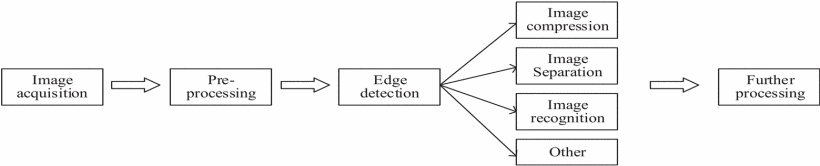
\includegraphics[width=1\textwidth]{Assets/Pipeline.png}
    \caption{Pipeline for image analysis techniques \cite{RTEdge}}
    \label{fig:pipeline}
\end{figure}

\cite{SoCImage, Aerial} follow a similar pipeline to Figure \ref{fig:pipeline}, with the image being captured by a camera module, and then processed by an FPGA though using differing image techniques.
The FPGA platform is optimal for any image detection tasks, as it can accelerate the required multiplication and addition operators separately - required for classical, and deep learning, based techniques \cite{ResourceEfficient}



\subsection{Convolutional Neural Networks and Deep Learning}
Convolutional neural networks (CNNs) are a type of artificial neural network that is primarily used for image detection.
Due to the lack of memory in low-end FPGA models, the CNN is optimal for an image processing task on SoC, as it has a low number of weights and biases relative to other neural networks \cite{Drowsiness}
The convolution operation requires a large number of multiply-accumulate (MAC) operations, and is the primary bottleneck in the performance of CNNs.
The operation must window over the entire image, and the number of MAC operations is proportional to the size of the image and the number of filters in the layer.
Hence, the CNN is computationally intensive, demanding a significant quantity of operations for high accuracy \cite{Linear}.
However, the proceeding \cite{Drowsiness} article found that the use of an embedded makes the implementation CNN less challenging on the FPGA platform, as the network can be designed in a systems language such as C.
This can then be compiled and translated into machine code, as there exists a toolchain for RISC-V.

Similar works for image-analysis using different neural network architectures have also been implemented using FPGA hardware.
\cite{Yolo, SparseYolo } demonstrates a hardware implementation of the You Only Look Once (YOLO) algorithm using a Xilinx Virtex-7 FPGA. 
Like the CNN hardware implementations, the architecture is focused on accelerating the convolution operation - and is a common denominator in the performance neural networks in hardware.
This acceleration is not specific to the convolution operator, and can be applied to any intensive operation in the network as the FPGA has little overhead on each operator when compared to traditional platforms \cite{Overhead}.
This is corroborated by \cite{Throughput}, which found that the implementation of hybrid neural networks on a Xilinix Virtex-7 690T FPGA achieved 4.13 times higher throughput than state of the accelerators in 2019.

\subsection{RISC-V}
Instruction set architectures (ISAs) define the operations a processor can execute, but the majority of ISAs are proprietary. 
Reduced Instruction Set Computing (RISC) is a form of ISA which offers a simpler, more efficient design than the traditional Complex Instruction Set Computing (CISC) ISAs - such as the prevalent x86 instruction set \cite{Arm}.
Arm and RISC-V are the two most prominent RISC ISAs, with Arm being the most widely used in embedded systems but with RISC-V offering royalty-free licensing and an open-source nature.
The lack of licensing fees and the open-source nature of RISC-V has led to its increasing popularity in the embedded systems domain \cite{Neutron}.
It is estimated that the number of chips utilising RISC-V technology "will grow 73.6 percent per year to 2027, when there will be some 25 billion AI chips produced, accounting for US \$291 billion in revenue" \cite{Drowsiness}.

There exists a number of FPGA implementations to create softcore processors using the RISC-V ISA \cite{RISCFPGA}. 
The 2023 paper \cite{Neutron} demonstrates a RISC-V implementation of the NEORV32 core, using a Wishbone bus interface. 
The authors selected the NEORV32 core due to the vendor-agnostic and platform independency, and the project being highly documented.
The softcore nature allows for the implementation details to be customised to the specific application, such that the core can be adapted to the specific use case \cite{DCT}. The NEORV32 processors offers a system-on-chip (SoC) Harvard architecture, with a 32-bit RISC-V processor, and a range of peripherals.
It supports UART, SPI, standard GPIO and the Wishbone b4 external bus interface for SoC connectivity \cite{NEORV32}.

As it is an open-source ISA, RISC-V has the added benefit of being extensible and modular \cite{Cryptography}, allowing for instructions to be added to the processor.
\cite{Reconfigurable} utilises this to create custom instructions within the RISC-V ISA to accelerate the expensive convolution operation for a CNN.

\subsection{Field-Programmable Gate Arrays}
Field Programmable gate arrays (FPGAs) provide flexible compute resources that can be reconfigured to suit a wide range of applications.
Similar to graphics processing units (GPUs), FPGAs offer parallel processing capabilities, but with the added benefit of reconfigurability \cite{Parallelism}.
The ability to develop custom logic designs is not unique to FPGAs, as application-specific integrated circuits (ASICs) also offer this capability, but FPGAs offer a faster development cycle and lower cost for low-volume production.
Hence, FPGA technology is optimal for edge applications on images due to the parallelised pipeline structure, which enables high-speed processing of large amounts of image data, and it's high processing speed ensures real-time image data processing \cite{Video}.

FPGAs have been studied extensively in the field of image detection, as replacements to existing hardware infrastructures. 
The most common application is to accelerate the convolution operation using the parallel processing capabilities of FPGAs. 

Figure \ref{fig:gradient} shows an implemention of a hardware-accelerated edge-detection algorithm for video images, using the Intel Cyclone IV FPGA platform direct from a camera module. 
This requires a camera module, FPGA and uses a VGA monitor to display the output - but does not use a softcore processor. 

\begin{figure}[h]
    \centering
    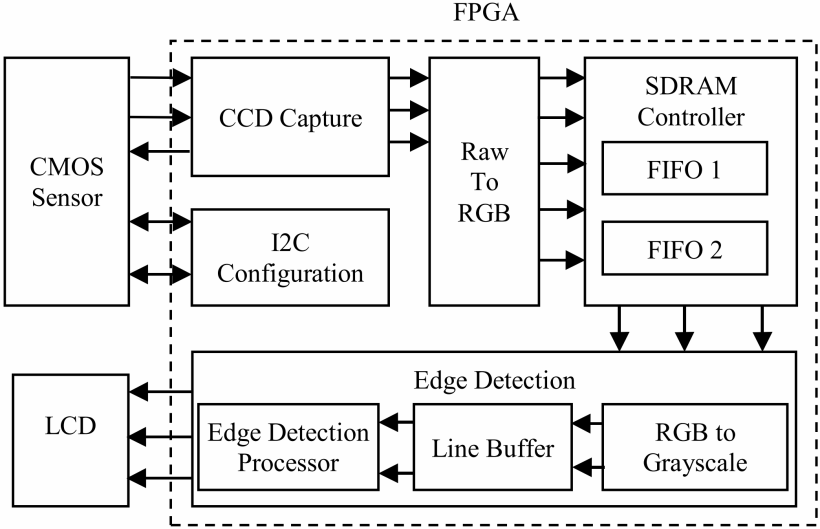
\includegraphics[width=1\textwidth]{Assets/Gradient.png}
    \caption{Video detection FPGA pipeline \cite{Gradient}}
    \label{fig:gradient}
\end{figure}

This pipeline has the core advantage over traditional CPU architectures which are serially structured, as it can perform the operations in hardware and in parallel. 
Hence, an image processing system employing an FPGA as the primary control chip is better suited to the low-latency and high speed demands of real-time image processing \cite{RTEdge}.